%% LaTeX Beamer presentation template (requires beamer package)
%% see http://bitbucket.org/rivanvx/beamer/wiki/Home
%% idea contributed by H. Turgut Uyar
%% template based on a template by Till Tantau
%% this template is still evolving - it might differ in future releases!

\documentclass{beamer}

\mode<presentation>
{
\usetheme{Warsaw}

\setbeamercovered{transparent}
}

\usepackage[english]{babel}
\usepackage[latin1]{inputenc}

% font definitions, try \usepackage{ae} instead of the following
% three lines if you don't like this look
\usepackage{mathptmx}
\usepackage[scaled=.90]{helvet}
\usepackage{courier}


\usepackage[T1]{fontenc}


\title{PyWPS 4.0 - Advanced Features}

%\subtitle{}

% - Use the \inst{?} command only if the authors have different
%   affiliation.
\author{L.~M.~de~Sousa\inst{1} \and J.~M.~de~Jesus\inst{2}}
%\author{\inst{1}}

% - Use the \inst command only if there are several affiliations.
% - Keep it simple, no one is interested in your street address.
\institute[Universities of]
{
\inst{1}%
Eawag - Swiss Federal Institute of Aquatic Science and Technology
\and
\inst{2}%
GeoCAT}

\date{$10^{th}$ of May / GeoPython Conference 2017}


% This is only inserted into the PDF information catalog. Can be left
% out.
\subject{Talks}



% If you have a file called "university-logo-filename.xxx", where xxx
% is a graphic format that can be processed by latex or pdflatex,
% resp., then you can add a logo as follows:

% \pgfdeclareimage[height=0.5cm]{university-logo}{university-logo-filename}
% \logo{\pgfuseimage{university-logo}}



% Delete this, if you do not want the table of contents to pop up at
% the beginning of each subsection:
\AtBeginSubsection[]
{
\begin{frame}<beamer>
\frametitle{Outline}
\tableofcontents[currentsection,currentsubsection]
\end{frame}
}

% If you wish to uncover everything in a step-wise fashion, uncomment
% the following command:

%\beamerdefaultoverlayspecification{<+->}

\begin{document}

\begin{frame}
\titlepage
\end{frame}

\begin{frame}
\frametitle{Outline}
\tableofcontents
% You might wish to add the option [pausesections]
\end{frame}

% %%%%%%%%%%%%%%%%%%%%%%%%%%%%%%%%%%%%%%%%%%%%%%%%%%%%%%%%%%%%%%%%%%%%%%%%%%%%%
\section{Introduction}

%\subsection[Short First Subsection Name]{First Subsection Name}

% -----------------------------------------------
\begin{frame}
\frametitle{PyWPS 4.0 is finally here}
%\framesubtitle{Subtitles are optional}

\begin{itemize}
  \item Over three years in development \pause
  \item Relevant contributions by over a dozen individuals \pause
  \item New licence: MIT \pause
  \item OSGeo acreditation around the corner \ldots \pause
\end{itemize}
\end{frame}

% \begin{frame}
% \frametitle{}
% 
% % You can create overlays
% \begin{itemize}
%   \item using the \texttt{pause} command:
%   \begin{itemize}
%     \item First item.
%     \pause
%     \item Second item.
%   \end{itemize}
%   \item using overlay specifications:
%   \begin{itemize}
%     \item<3-> First item.
%     \item<4-> Second item.
%   \end{itemize}
%   \item using the general \texttt{uncover} command:
%   \begin{itemize}
%     \uncover<5->{\item First item.}
%     \uncover<6->{\item Second item.}
%   \end{itemize}
% \end{itemize}
% \end{frame}



% -----------------------------------------------
\begin{frame}
\frametitle{What is PyWPS?}

\begin{itemize}
  \item An implementation of the OGC Web Processing Service
standard
\item Coded on the Python language (researcher friendly)
\item Started in the Spring of 2006
\item Supports all available tools in Python for geospatial operations
\item http://pywps.org
  
\end{itemize}
\end{frame}


% -----------------------------------------------
\begin{frame}
\frametitle{What PyWPS is not}

\begin{itemize}
  \item Complicated
  \item A client
  \item A GUI or any other user interface
  \item a server with pre-installed processes
  \item 
  
\end{itemize}
\end{frame}



% -----------------------------------------------
\begin{frame}
\frametitle{What is PyWPS good for?}

\begin{itemize}
  \item Make your models available to the world
  \item Enables remote processing of complex and/or length models 
  \item Guarantee model inputs fit basic requirements (e.g. type, quantity)
  \item Guarantee interoperability of model inputs and outputs
  \begin{itemize}
    \item using the OGC data standards
	\item 
  \end{itemize}
\end{itemize}
\end{frame}


% %%%%%%%%%%%%%%%%%%%%%%%%%%%%%%%%%%%%%%%%%%%%%%%%%%%%%%%%%%%%%%%%%%%%%%%%%%%%%
\section{OGC Web Processing Service}

% -----------------------------------------------
\begin{frame}
\frametitle<presentation>{The OGC Web Processing Service}

\begin{itemize}
\item OGC open web standard for remote geo-spatial processing.
\item Integrated with web data services: \textbf{WFS}, \textbf{WCS}.
\item Three basic requests:
\begin{itemize}   
      \item  \textit{GetCapabilities}
      \item  \textit{DescribeProcess}
      \item  \textit{Execute}
\end{itemize}
\item Three basic input/output classes:
\begin{itemize}   
      \item  \textit{Literal}
      \item  \textit{Complex} - for geo-spatial data and services
      \item  \textit{BoundingBox} - for geo-spatial data extent
\end{itemize}
\end{itemize}
\end{frame}



% -----------------------------------------------
\begin{frame}
\frametitle<presentation>{The OGC Web Processing Service}

  \begin{figure}[ht]
   \centering
   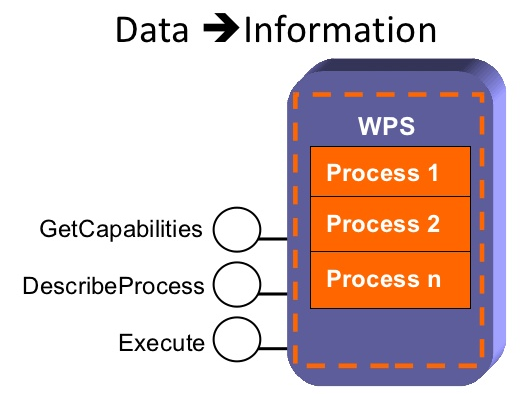
\includegraphics[height=6cm]{figures/WPS}
  \end{figure}

\centering
\footnotesize{http://www.slideshare.net/TheodorFoerster/restful-web-processing-service}

\end{frame}


% %%%%%%%%%%%%%%%%%%%%%%%%%%%%%%%%%%%%%%%%%%%%%%%%%%%%%%%%%%%%%%%%%%%%%%%%%%%%%
\section*{Logging and SQLAlchemy}

% -----------------------------------------------
\begin{frame}
\frametitle<presentation>{Accessing logs in previous versions}

\end{frame}

% -----------------------------------------------
\begin{frame}
\frametitle<presentation>{Logs in PyWPS 4.0}

\end{frame}

% -----------------------------------------------
\begin{frame}
\frametitle<presentation>{Easy to configure}

\end{frame}


% -----------------------------------------------
\begin{frame}
\frametitle<presentation>{SQLAlchemy}

\end{frame}


% %%%%%%%%%%%%%%%%%%%%%%%%%%%%%%%%%%%%%%%%%%%%%%%%%%%%%%%%%%%%%%%%%%%%%%%%%%%%%
\section*{Deployment with Nginx}


% -----------------------------------------------
\begin{frame}
\frametitle<presentation>{PyWPS 4.0 is a Flask application}

\begin{itemize}
  \item PyWPS 4.0 developed with WSGI in mind
  \item Distributed by default as a Flask application
  \item It can be run directly on Flash - not advisable
  \begin{itemize}
    \item no request concurrency
    \item no request queueing
    \item Flask is primarily meant for development
  \end{itemize}
  \item PyWPS 4.0 can be run on Nginx - not advisable
  \begin{itemize}
    \item 
  \end{itemize} 
\end{itemize}

\huge{Confused ?}

\end{frame}
% %%%%%%%%%%%%%%%%%%%%%%%%%%%%%%%%%%%%%%%%%%%%%%%%%%%%%%%%%%%%%%%%%%%%%%%%%%%%%
\section*{Summary}

\begin{frame}
\frametitle<presentation>{Summary}

\begin{itemize}
  \item The \alert{first main message} of your talk in one or two lines.
\end{itemize}

% The following outlook is optional.
\vskip0pt plus.5fill
\begin{itemize}
  \item Outlook
  \begin{itemize}
    \item Something you haven't solved.
    \item Something else you haven't solved.
  \end{itemize}
\end{itemize}
\end{frame}

\end{document}
